\chapter{Introduction}\label{ch:intro}
\section{Point processes} \label{sec:point_processes}
Within the large framework of complex systems, stochastic processes lend us a hand to decypher properties of living systems, bridging randomness with structured behaviour.
This processes are used to model the dynamics of systems which evolve randomly in time. This is why they are ideal for describing natural phenomena such as 
the spread of diseases \cite{Chowell}, social networks \cite{castellano2009statistical} or ecological systems \cite{azaele2016statistical}. Mathematically, a stochastic process
is a collection of random variables \cite{McKane}, generally ordered in time $ \{X_t\}_{t \in T} $, where $t$ is the time and $X_t$ is the system state at time $t$. $T$ is the time index set, 
which can be discrete or continuous, in this work we will focus on the discrete case because we are interested in the study of point (Hawkes) processes for modeling neurons. 

Point processes are a type of stochastic process that describe the occurrence of events in time or space. We will be interested in time point processes because 
we are going to model the spiking activity of neurons. For our purposes, they will be characterized by two parameters, the time of occurrence
of the events $t_k$ and the intensity or rate of occurrence of these events $\lambda$. This rate tell us how likely is that an event occurs at time $t$ given the history of the process 
(probability density function, PDF) as pictured in Figure \ref{f:point_process}.

\begin{figure}[H]
    \centering
    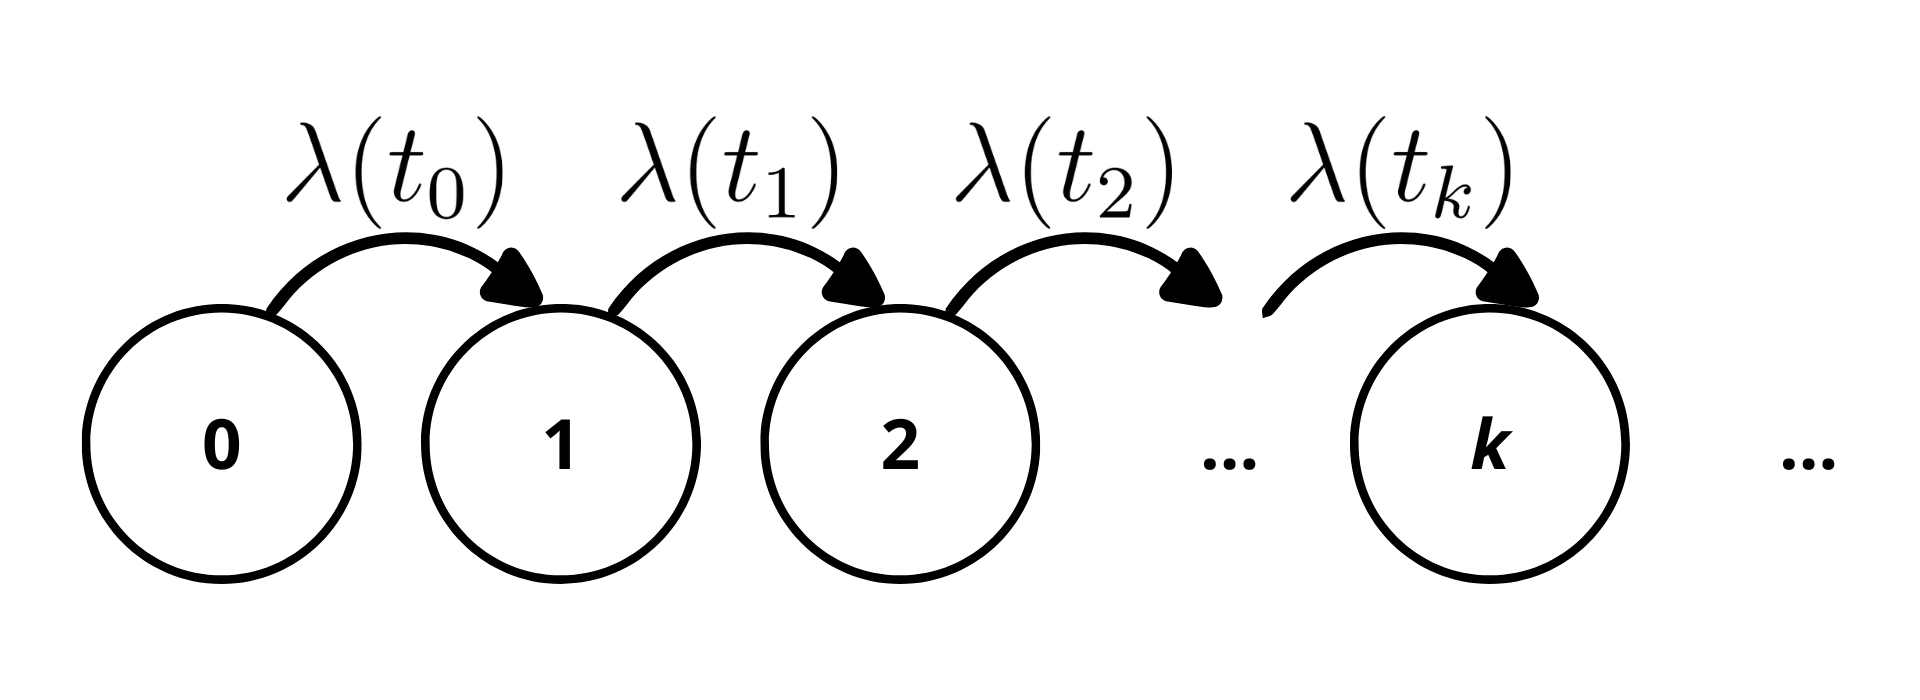
\includegraphics[width=0.85\textwidth]{Point process.png}
    \caption{Representation of a point process. The intensity function $\lambda(t)$ is a time-dependent function.}
    \label{f:point_process}
\end{figure}

In general, the rate is a function of the history of the process, which makes the process non-Markovian, but in our case, it will be a Markovian process, which means that the rate depends 
only on the last event that occurred as we will see. An example of a Markovian point process is the Poisson process, which is a simple and one of the most studied point processes because 
they are present in many everyday situations such as the arrival of customers at a store, occurrence of defects on a Production line. They are also present in some physics phenomena,
for instance, the decay of radioactive particles or the arrival of photons at a detector. These processes are characterized by a rate of occurrence of events $\lambda$.
The dynamics of these processes are described by the Poisson distribution which is the probability distribution of a random variable $N$ such that the probability that $N= n$ is:
\begin{equation}
    P(N=n) = \dfrac{\lambda^n}{n!}e^{-\lambda}.
    \label{eq: Probabilidad proceso de Poisson homogéneo}
\end{equation}
Furthermore, the mean value and the variance of the distribution are also equal to $\lambda$. Poisson processes can be homogeneous or inhomogeneous, depending on whether the rate is constant
or time-dependent. In Figure \ref{f:poisson} we can see an example of a homogeneous Poisson process.

\begin{figure}[H]
    \centering
    \includegraphics[width=0.95\textwidth]{Poisson probabilidad y nº eventos.png}
    \caption{Left: event number in time for different rates. Right: Probability of having a certain number of events for different rates.}
    \label{f:poisson}
\end{figure}

\section{Hawkes processes} \label{sec:Hawkes_processes}

On the other hand if we consider a non-homogeneous Poisson process, the rate is a function of time, $\lambda(t)$, which is the case of the Hawkes process. The rate can be written in several 
ways \cite{notarmuzi2021percolation,kanazawa2021ubiquitous,dassios2013exact,laub2021elements}. We will use the the expression from \cite{notarmuzi2021percolation}:

\begin{equation}
    \lambda(t|t_1, \ldots, t_k) = \mu + n\sum_{i=1}^k \phi (t-t_i),
    \label{eq: Hawkes rate}
\end{equation}

where $\mu$ is the background rate of a homogeneous Poisson process, $n$ is a parameter that controls the strength the self-excitation, and $\phi(t)$ is the kernel function that
describes the influence of the past events on the rate of occurrence of the events. The kernel function is a non-negative and monotonically non-increasing function that integrates to 1.
Typical choices for the kernel function are the exponential or the power-law functions. In this work we will focus on the exponential kernel. 
From Eq \ref{eq: Hawkes rate} we can see that the rate depends on the history of the process, making it non-Markovian in general, but with an exponential kernel, the process becomes
Markovian. The kernel function can be written as: $\phi(t)=\sum_{t_i<t}\alpha e^{-\beta(t-t_i)}$ so the rate becomes:

\begin{equation}
    \begin{split}
        \lambda(t) &= \mu + \sum_{t_i<t}\alpha e^{-\beta(t-t_i)}\\
        &= \mu + \sum_{\underbrace{t_i<t_k}_{t_k\text{: last event}}}\alpha e^{-\beta(t-t_k+t_k-t_i)}\\
        &= \mu + e^{-\beta(t-t_k)}\underbrace{\sum_{t_i<t_k}\alpha e^{-\beta(t_k-t_i)}}_{\lambda(t_k)}\\
        &= \mu + e^{-\beta(t-t_k)}\left( \lambda(t_k)-\mu+n \right).
    \end{split}
    \label{eq: Hawkes rate exponential becomes Markovian}
\end{equation}

Where we have used the following expression for the rate of the Hawkes process at time $t_k$:

\begin{equation}
    \lambda(t_k) =\mu+\sum_{t_i<t_k}\alpha e^{-\beta(t_k-t_i)}\Rightarrow\sum_{t_i<t_k}\alpha e^{-\beta(t_k-t_i)} = \lambda(t_k)-\mu+\alpha
    \label{eq: Hawkes rate at event time}
\end{equation}

Despite being a Markovian process, it is still an inhomogeneous Poisson process because the rate is not constant. In addition, it is a self-exciting process, which means that the occurrence
of an event increases the probability of the occurrence of another event. This is why it is used to model the spiking activity of neurons, where the occurrence of a spike increases the
probability of the occurrence of another spike. This self-excitation will enable the appearance of bursts of activity that we will measure. The parameters chosen for the kernel function 
will be $\alpha=\beta=1$ and we will vary the background rate $\mu$ from values much smaller than 1 to values greater than 1. In Figures \ref{f: Hawkes rate} and \ref{f: Hawkes rate 2}
we can see typical diagrams of Hawkes processes with these parameters.

\begin{figure}[H]
    \centering
    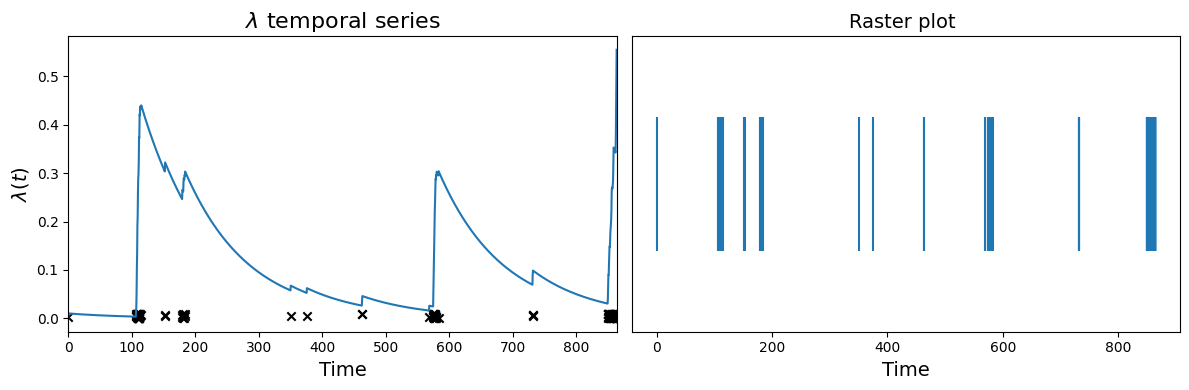
\includegraphics[width=0.95\textwidth]{Hawkes mu 0.01.png}
    \caption{On the left, a temporal series of $K=150$ events of a Hawkes process with $\mu=0.01$, on the right, a raster plot of the same process.}
    \label{f: Hawkes rate}
\end{figure}

\begin{figure}[H]
    \centering
    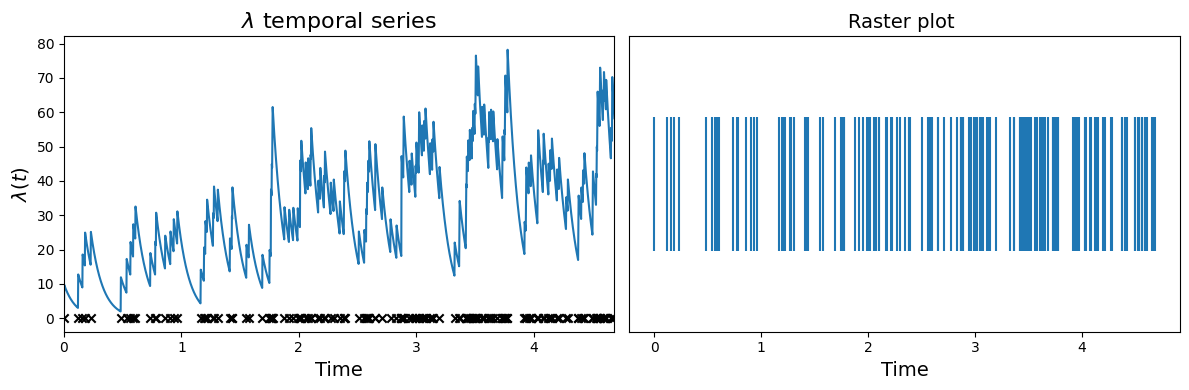
\includegraphics[width=0.95\textwidth]{Hawkes mu 10.png}
    \caption{On the left, a temporal series of $K=150$ events of a Hawkes process with $\mu=0.01$, on the right, a raster plot of the same process.}
    \label{f: Hawkes rate 2}
\end{figure}

As shown in Figure \ref{f: Hawkes rate}, when the background rate is smaller than 1, events are less likely to occur, but when they do, they tend to form avalanches of activity thanks 
to the self-excitation. On the other hand, when the background rate is greater than 1, events occur more frequently, forming avalanches of activity more frequently and longer, as
shown in Figure \ref{f: Hawkes rate 2}. If we ignore the time of occurrence of the events and we focus only on the structure of $\lambda$ and therefore of the events, we can see that
the process with $\mu=0.01$ has a bursty structure, while the process with $\mu=10$ has a more regular structure. This phenomenon is exposed in Figures \ref{f: Hawkes rate burst} and
\ref{f: Hawkes rate burst 2}.

\begin{figure}[H]
    \centering
    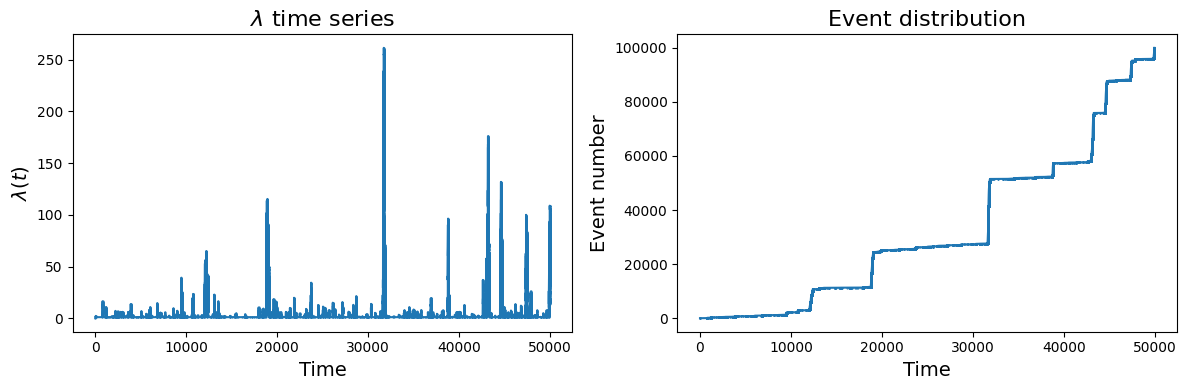
\includegraphics[width=0.95\textwidth]{Hawkes mu 0.01 events.png}
    \caption{First, a temporal series of $K=10^5$ events of a Hawkes process with $\mu=0.01$, on the right, the event distribution.}
    \label{f: Hawkes rate burst}    
\end{figure}

\begin{figure}[H]
    \centering
    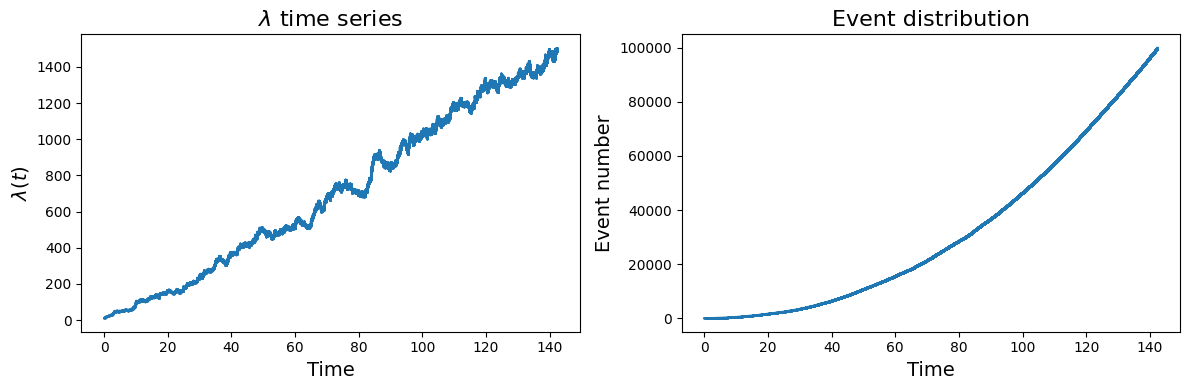
\includegraphics[width=0.95\textwidth]{Hawkes mu 10 events.png}
    \caption{First, a temporal series of $K=10^5$ events of a Hawkes process with $\mu=10$, on the right, the event distribution.}
    \label{f: Hawkes rate burst 2}    
\end{figure}

In most cases, the motivation of study of point processes is counting the events, but in our case we also are interested in the time of occurrence of the events
which will let us define bursts or avalanches of activity that we will use to describe the dynamics of the system. Additionally, 



Unless otherwise stated, $n=1$ HABLAR DE CRITICIDAD A PARTIR DE AQUÍ